
 % LuaLaTeX文書; 文字コーAドはUTF-8
 \documentclass[unicode,12pt, A4j]{ltjsarticle}% 'unicode'が必要
 %\usepackage{luatexja}% 日本語したい
 \usepackage{luatexja-fontspec}
 %\usepackage[hiragino-pron]{luatexja-preset}% IPAexフォントしたい(ipaex)
 \usepackage[hiragino-pron,deluxe,expert,bold]{luatexja-preset}
\usepackage{tikz}
\usetikzlibrary{arrows.meta}
\usetikzlibrary{calc}
\usepackage{ifthen}
 \usepackage[english]{babel}%多言語文書を作成する
 \usepackage{amsmath,amssymb}%標準数式表現を拡大する
 \usepackage{physics}
 \usepackage[subpreambles=true,sort=true]{standalone}
% \renewcommand{\kanjifamilydefault}{\gtdefault}% 既定をゴシック体に
 \usepackage{mhchem}
 % あとは欧文の場合と同じ




  \usepackage{caption}
  \usepackage[subrefformat=parens]{subcaption}
\title{東大数学理科後期1999年度}
\author{}
\date{}

\begin{document}
\maketitle

\section{問題1}

\begin{enumerate}
  \item $n$ を正の整数とする.$-\frac{\pi}{2} \le x \le \frac{\pi}{2}$ の範囲において
    \begin{align}
      f_n(x) = 
        \begin{cases} 
          \frac{\sin nx}{\sin x} & -\frac{\pi}{2} \le x \le \frac{\pi}{2},x \ne 0 \\ 
          c_n & x = 0 
        \end{cases} 
      \end{align}
とおくことにより定義される関数 $f_n(x)$ が,$x=0$ で連続となるように定数 $c_n$ の値を定めよ.  
  \item $f_3(x)$ を $\cos x, \cos 2x$ 等を用いて表せることを示し,定積分
\begin{align}
  \int_{-\frac{\pi}{2}}^{\frac{\pi}{2}} f_3(x) dx   
\end{align}
の値を求めよ.
  \item 任意の正の整数 $n$ に対して,定積分
\begin{align}
 \int_{-\frac{\pi}{2}}^{\frac{\pi}{2}} f_{2n+1}(x) dx   
\end{align}
の値を求めよ.
\end{enumerate}

\section{問題2}
座標平面上の原点を $O(0,0)$ とする.また,$x$ 座標および $y$ 座標がともに整数であるような点を格子点という.

\begin{enumerate}
 \item $t$ を正の実数とする.点 $P(-1, 0)$ を通り,傾きが $t$ の直線と単位円 $x^2 + y^2 = 1$ との $P$ 以外の交点を $Q(t)$ とする.$Q(t)$ の座標を求めよ.つぎに,$0 < s < t$ を満たす2つの実数 $s, t$ に対し,線分 $Q(s)Q(t)$ の長さを求めよ.
 \item $\angle Q(s)PO = \alpha, \angle Q(t)PO = \beta$ とし,
 \begin{align}
   u = \tan \frac{\alpha}{2}, \quad v = \tan \frac{\beta}{2}   
 \end{align}
とおく.もし $u, v$ がともに有理数ならば,線分 $Q(s)Q(t)$ の長さもまた有理数となることを示せ.
 \item 任意に与えられた3以上の整数 $n$ に対し,つぎの条件 (C1), (C2), (C3) をすべて満たす $n$ 個の異なる点 $A_1, A_2, \dots, A_n$ が,座標平面上に存在することを証明せよ.
\begin{itemize}
    \item[(C1)] $A_1, A_2, \dots, A_n$ はすべて格子点である.
    \item[(C2)] $A_1, A_2, \dots, A_n$ のどの異なる3点も一直線上にない.
    \item[(C3)] $A_1, A_2, \dots, A_n$ のどの異なる2点 $A_i, A_j$ に対しても,線分 $A_iA_j$ の長さは整数である.
\end{itemize}
\end{enumerate}

 

\section{問題3}
座標平面上にある3つの四角形 $ABCD$ と $A'B'C'D'$ が相似であるとは,対応する4つの頂点における内角がそれぞれ等しく,かつ対応する辺の長さの比がすべて等しいこととする.このとき,
\begin{align}
 \square ABCD \sim \square A'B'C'D' 
\end{align}
と書く.ただし,四角形 $ABCD$ と書くときには,4つの頂点 $A, B, C, D$ は図のように反時計回りに並んでいるものとし,また四角形は周および内部を込めて考えるものとする.

四角形$\text{A}_0 \text{B}_0 \text{C}_0 \text{D}_0$が与えられたとき,この四角形から出発して,任意の整数$n$に対して四角形$\text{A}_n \text{B}_n \text{C}_n \text{D}_n$を以下のように帰納的に定める.

\begin{itemize}
 \item[(I)] $n = 0$のときは,与えられた四角形$\text{A}_0 \text{B}_0 \text{C}_0 \text{D}_0$とする.
 \item[(II)] $n > 0$のときは,四角形$\text{A}_{n-1} \text{B}_{n-1} \text{C}_{n-1} \text{D}_{n-1}$まで定まったとして,四角形$\text{A}_n \text{B}_n \text{C}_n \text{D}_n$を
\begin{align}
\text{A}_n = \text{D}_{n-1}, \quad \text{B}_n = \text{C}_{n-1} \text{ かつ } \square\text{A}_n \text{B}_n \text{C}_n \text{D}_n \sim \square \text{B}_{n-1} \text{C}_{n-1} \text{D}_{n-1} \text{A}_{n-1}  
\end{align}
となる四角形として定める.
 \item[(III)] $n < 0$のときは, $0, -1, \dots, n+1$と負の向きに進んで,四角形$\text{A}_{n+1} \text{B}_{n+1} \text{C}_{n+1} \text{D}_{n+1}$まで定まったとして,四角形$\text{A}_n \text{B}_n \text{C}_n \text{D}_n$を
\begin{align}
 \text{D}_n = \text{A}_{n+1}, \quad \text{C}_n = \text{B}_{n+1} \text{ かつ } \square \text{A}_n \text{B}_n \text{C}_n \text{D}_n \sim \square \text{B}_{n+1} \text{C}_{n+1} \text{D}_{n+1} \text{A}_{n+1} 
\end{align}
となる四角形として定める.
\end{itemize}

こうして定まった四角形$\text{A}_n \text{B}_n \text{C}_n \text{D}_n$を$K_n$と書くことにする.

さて,座標平面上の$3$点
\begin{align}
 \text{A}_0(2, 1), \quad \text{B}_0(8, 4), \quad \text{P}(4, 12) 
\end{align}
を与える.原点を$\text{O}$とし,線分$\text{OP}$上に原点以外の1点$\text{C}_0$をとる.点$\text{A}_0$から線分$\text{B}_0 \text{C}_0$に平行に引いた直線と,線分$\text{OP}$との交点を$\text{D}_0$とする.このようにして定まる四角形$\text{A}_0 \text{B}_0 \text{C}_0 \text{D}_0$から出発して,上記のようにして得られる四角形の系列
\begin{align}
 \dots, K_{-2}, K_{-1}, K_0, K_1, K_2, \dots 
\end{align}
について考える.
\begin{enumerate}
 \item $\angle \text{D}_0\text{D}\text{P}$を求めよ.
 \item 線分$\text{OP}$上のある点$\text{C}_0$を与え,それにより定まる四角形$\text{A}_0 \text{B}_0 \text{C}_0 \text{D}_0$から出発して,四角形の系列$\dots, K_{-2}, K_{-1}, K_0, K_1, K_2, \dots$を作ったところ,ある0でない整数$n$が存在して,$K_n = K_0$となったという.このとき,点$\text{C}_0$の座標を求めよ.また,$K_n = K_0$となる整数$n$の値をすべて求めよ.
 \item 線分$\text{OP}$上のある点$\text{C}_0$を与え,それにより定まる四角形$\text{A}_0 \text{B}_0 \text{C}_0 \text{D}_0$から出発して,四角形の系列$\dots, K_{-2}, K_{-1}, K_0, K_1, K_2, \dots$を作ったところ,これらの四角形が座標平面において原点を除いた部分を,辺と頂点以外には互いに重なることなく,すき間なくおおったという.このような性質をもつ点$\text{C}_0$をすべて求め,それらの座標を記せ.またそれらの場合のおのおのについて,点$(100, 50)$が$K_n$に含まれるような整数$n$の値をすべて求めよ.
\end{enumerate}

\begin{figure}[h]
\centering
 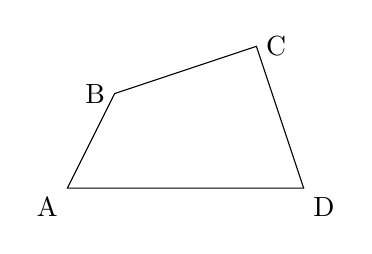
\begin{tikzpicture}[scale=0.6]
\draw (0,0) -- (5,0) -- (4,3) -- (1,2) -- cycle;
\node[left] at (1,2) {B};
\node[below left] at (0,0) {A};
\node[below right] at (5,0) {D};
\node[right] at (4,3) {C};
\end{tikzpicture}
\end{figure}





\end{document}